
% !TEX encoding = UTF-8 Unicode 
% !TEX root = FieldGuide.tex

\clearpage
\Sec{Limits}
\label{sec:Limits}
\index{limits}

\SSec{Exponential function limit}
\label{sec:Limits:exp}
A common and important limit is 
\[
\lim_{c\rightarrow+\infty} \Left(1 + \frac{x}{c} \Right)^{a c} = e^{a x} \ . \checked
\notag
\]
In particular, the $X$-exponential distributions are the exponential limit of Weibullized distributions.

\begin{align*}
\lim_{\beta\rightarrow\infty} f\Bigl[ \bigl(\frac{x-a}{s}\bigr)^{\beta} \Bigr]
&= \lim_{\beta\rightarrow \infty} f\Bigl[\bigl(1 - \frac{1}{\beta} \frac{x-\pLoc }{ \pScale}\bigr)^{\beta}  \Bigr] =  f\Bigl[ e^{-\frac{x-\pLoc}{\pScale}} \Bigr] \checked
\\ & \qquad (a = \pLoc + \beta\pScale, \ s = - \beta \pScale) 
\checked
\end{align*}
\begin{align*}
\opr{Exp}(x\given a,\theta) &=  \lim_{\beta\rightarrow\infty} \opr{PowerFn} (x\given a+\beta\theta,-\beta\theta,\beta)
\checked
\\
\opr{GammaExp}(x\given \nu, \lambda, \alpha) &=  \lim_{\beta\rightarrow\infty} \opr{Amoroso}(x\given \nu+\beta \lambda,-\beta \lambda, \alpha,\beta)
\checked
\\
\opr{Gamma}(x\given a,s,\alpha) &= \lim_{\beta\rightarrow\infty} \opr{UnitGamma}(x\given a+\beta s,-\beta s, \alpha,\beta) 
\checked
\\
\opr{BetaExp}(x\given \pLoc, \pScale, \alpha, \gamma) 
& = \lim_{\beta\rightarrow\infty } \opr{GenBeta}(x\given \pLoc+\beta\lambda, -\beta\pScale, \alpha, \gamma, \beta) 
\checked
\\
  \opr{BetaLogistic}(x\given \pLoc, \pScale, \alpha, \gamma)  &=
 \lim_{\beta\rightarrow\infty}  \opr{GenBetaPrime}(x\given \pLoc+\beta\pScale, -\beta \pScale, \alpha, \gamma, \beta)  
\checked
\\
\opr{Normal}(x\given \mu, \sigma) & =   \lim_{\beta\rightarrow\infty} \opr{LogNormal}(x\given \mu + \beta\sigma, -\beta\sigma, \beta) \checked
\end{align*}



We can play the same trick with the $\gamma$ shape parameter in the beta  and beta prime families.
\begin{align*}
\lim_{\gamma \rightarrow\infty} f\Bigl[ \bigl(1- \Left(\frac{x-a}{s}\Right)^{\beta} \bigr)^{\gamma-1} \Bigr]
& = \lim_{\gamma \rightarrow\infty} f\Bigl[ \bigl(1-\frac{1}{\gamma} \Left(\frac{x-a}{\theta}\Right)^{\beta} \bigr)^{\gamma-1} \Bigr]
\checked
\\ & =  f\Bigl[ e^{-(\frac{x-a}{\theta})^\beta} \Bigr] 
\qquad s = \theta \gamma^{\frac{1}{\beta}} \checked
\end{align*}
% 
\begin{align*}
\opr{Amoroso}(x\given a,\theta,\alpha, \beta)   & =
\lim_{\gamma\rightarrow\infty} \opr{GenBeta}(x\given a, \theta \gamma^{\frac{1}{\beta}} ,\alpha, \gamma, \beta )
\checked
\\
\opr{Gamma}(x\given a, \theta,\alpha)   \
& =  \lim_{\gamma\rightarrow\infty} \opr{Beta}(x\given a, \theta \gamma ,\alpha, \gamma ) \checked
\end{align*}



\begin{align*}
\lim_{\gamma \rightarrow\infty} f\Bigl[ \bigl(1+ \Left(\frac{x-a}{s}\Right)^{\beta} \bigr)^{-\alpha-\gamma} \Bigr]
& = \lim_{\gamma \rightarrow\infty} f\Bigl[ \bigl(1+\frac{1}{\gamma} \Left(\frac{x-a}{\theta}\Right)^{\beta} \bigr)^{-\alpha-\gamma} \Bigr] \checked
\\ & =  f\Bigl[ e^{-(\frac{x-a}{\theta})^\beta} \Bigr] 
\qquad s = \theta \gamma^{\frac{1}{\beta}} \checked
\end{align*}
%
\begin{align*}
\opr{Amoroso}(x \given a,\theta,\alpha, \beta)  & =
\lim_{\gamma\rightarrow\infty} \opr{GenBetaPrime}(x\given a, \theta \gamma^{\frac{1}{\beta}} ,\alpha, \gamma, \beta ) 
\checked
\\
\opr{Gamma}(x\given 0, \theta,\alpha)  
& =
\lim_{\gamma\rightarrow\infty} \opr{BetaPrime}(x\given 0, \theta \gamma ,\alpha, \gamma ) \checked
\\
\opr{InvGamma}(x\given \theta,\alpha) 
& =
\lim_{\gamma\rightarrow\infty} \opr{BetaPrime}(x\given 0, \theta/ \gamma ,\alpha, \gamma )  \checked
\end{align*}

Essentially the same limit takes the beta-exponential and beta-logistic distributions to the Gamma-Exponential distribution. 
\[
\notag
\opr{GammaExp}(x\given \nu, \lambda, \alpha)  & =
{\lim_{\gamma\rightarrow\infty} \opr{BetaExp}(x \given \nu+\lambda/\ln\gamma, \lambda, \alpha, \gamma)  }
\checked
\\
\notag
\opr{GammaExp}(x\given \nu, \lambda, \alpha)  & =
{\lim_{\gamma\rightarrow\infty} \opr{BetaLogistic}(x \given \nu+\lambda/\ln\gamma,\lambda, \alpha, \gamma)  }
\checked
\\
\notag
\opr{Gumbel}(x\given \nu, \lambda)  & =
{\lim_{\gamma\rightarrow\infty} \opr{ExpExp}(x \given \nu+\lambda/\ln\gamma, \lambda, \gamma)  }
\\
\notag
\opr{Gumbel}(x\given \nu, \lambda)  & =
{\lim_{\gamma\rightarrow\infty} \opr{BurrII}(x \given \nu+\lambda/\ln\gamma,\lambda, \gamma)  }
\]





\SSec{Logarithmic function limit}
\index{logarithmic function limit}
\[
\lim_{c\rightarrow0} \frac{x^c -1}{c} = \ln x
\notag \checked
\]

\[
\opr{UnitGamma}(x\given a, s, \gamma,\beta) =
\lim_{\alpha\rightarrow\infty } \opr{GenBeta}(x\given a,s,\alpha, \gamma,\beta/\alpha)
\checked 
\notag
\]




\SSec{Gaussian function limit}
\index{Gaussian function limit}
% From Wolfram Alpha
% limit  (1-z/{sqrt{c}} )^c exp(z sqrt{c} ) as c->infinity
\[
\lim_{c \rightarrow \infty} e^{-z \sqrt{c}}  \bigl( 1+\frac{z}{\sqrt{c}} \bigr)^c = e^{-\half z^2}
\checked
\notag
\]

\begin{align*}
\opr{LogNormal} (x\given a, \vartheta, \sigma) & =
\lim_{\gamma\rightarrow\infty} \opr{UnitGamma} (x\given a, \vartheta e^{ \sigma\sqrt{\gamma}}, \alpha, \tfrac{\sqrt{\gamma}}{\sigma} )
\checked
\\
\opr{Normal}(x\given \mu,\sigma)   & = 
\lim_{\alpha\rightarrow\infty} \opr{Gamma} (x\given \mu- \sigma\sqrt{\alpha}, \tfrac{\sigma}{\sqrt{\alpha}}, \alpha)
\checked
\\
\opr{Normal}(x\given \mu,\sigma)   & = 
\lim_{\alpha\rightarrow\infty} \opr{InvGamma} (x\given \mu-\sigma\sqrt{\alpha}, \sigma \alpha^{\tfrac{3}{2}}, \alpha)
\checked
\end{align*}


% This is for Amoroso
% Wolfram Alpha
% lim_(c->oo) (c+(c z)/sqrt(c)-c e^(z/sqrt(c))) = -z^2/2
\[
\lim_{c\rightarrow\infty} e^{c + c  \frac{z}{\sqrt{c}} - c e^{\frac{z}{\sqrt{c}}} }= e^{- \frac{z^2}{2}} \checked
\notag
\]

\[
\opr{LogNormal}(x\given a,\vartheta,\sigma)  & = \lim_{\alpha\rightarrow\infty} 
\opr{Amoroso}(x\given  a, \vartheta \alpha^{-\sigma\sqrt{\alpha} } , \alpha, \tfrac{1}{\sigma \sqrt{\alpha}})  
\notag \checked
\\
 \opr{Normal}(x\given \mu, \sigma) & = 
\lim_{\alpha\rightarrow\infty} \opr{GammaExp}(x\given  \mu+\sigma\sqrt{\alpha}\ln\alpha, \sigma\sqrt{\alpha},\alpha)
\checked
\notag
\]




\SSec{Miscellaneous limits}


\[
 \opr{InvGamma}(x\given \theta, \alpha) & =
 \lim_{v\rightarrow\infty} \opr{PearsonIV}(x\given 0,-\tfrac{\theta}{2 v}, \tfrac{\alpha+1}{2},v)
 \checked
 \notag
\]
See \secref{sec:PearsonIV}

\[
\opr{Normal}(x\given \mu,\sigma)   & = 
\lim_{m\rightarrow\infty} \opr{PearsonVII}( x\given \mu, \sigma\sqrt{2m},m)
\checked
\notag
\\
\opr{Normal}(x\given \mu,\sigma)   & = 
\lim_{\alpha\rightarrow\infty} \opr{CentralBeta}( x\given \mu, \sigma\sqrt{8\alpha},\alpha)
\checked
\notag
\]

\[
\opr{Laplace}(x\given \eta,\theta)   & = 
\lim_{\alpha\rightarrow 0} \opr{BetaLogistic}( x\given \eta, \theta\alpha, \alpha, \alpha)
\notag
\checked
\]



\definecolor{darkgreen}{RGB}{0,128,0}
\begin{figure*}
\caption[Limits and special cases of principal distributions]{Limits and special cases of principal distributions} 
%\label{PrincipalHierarchy}
\begin{center}
\scalebox{0.58} {
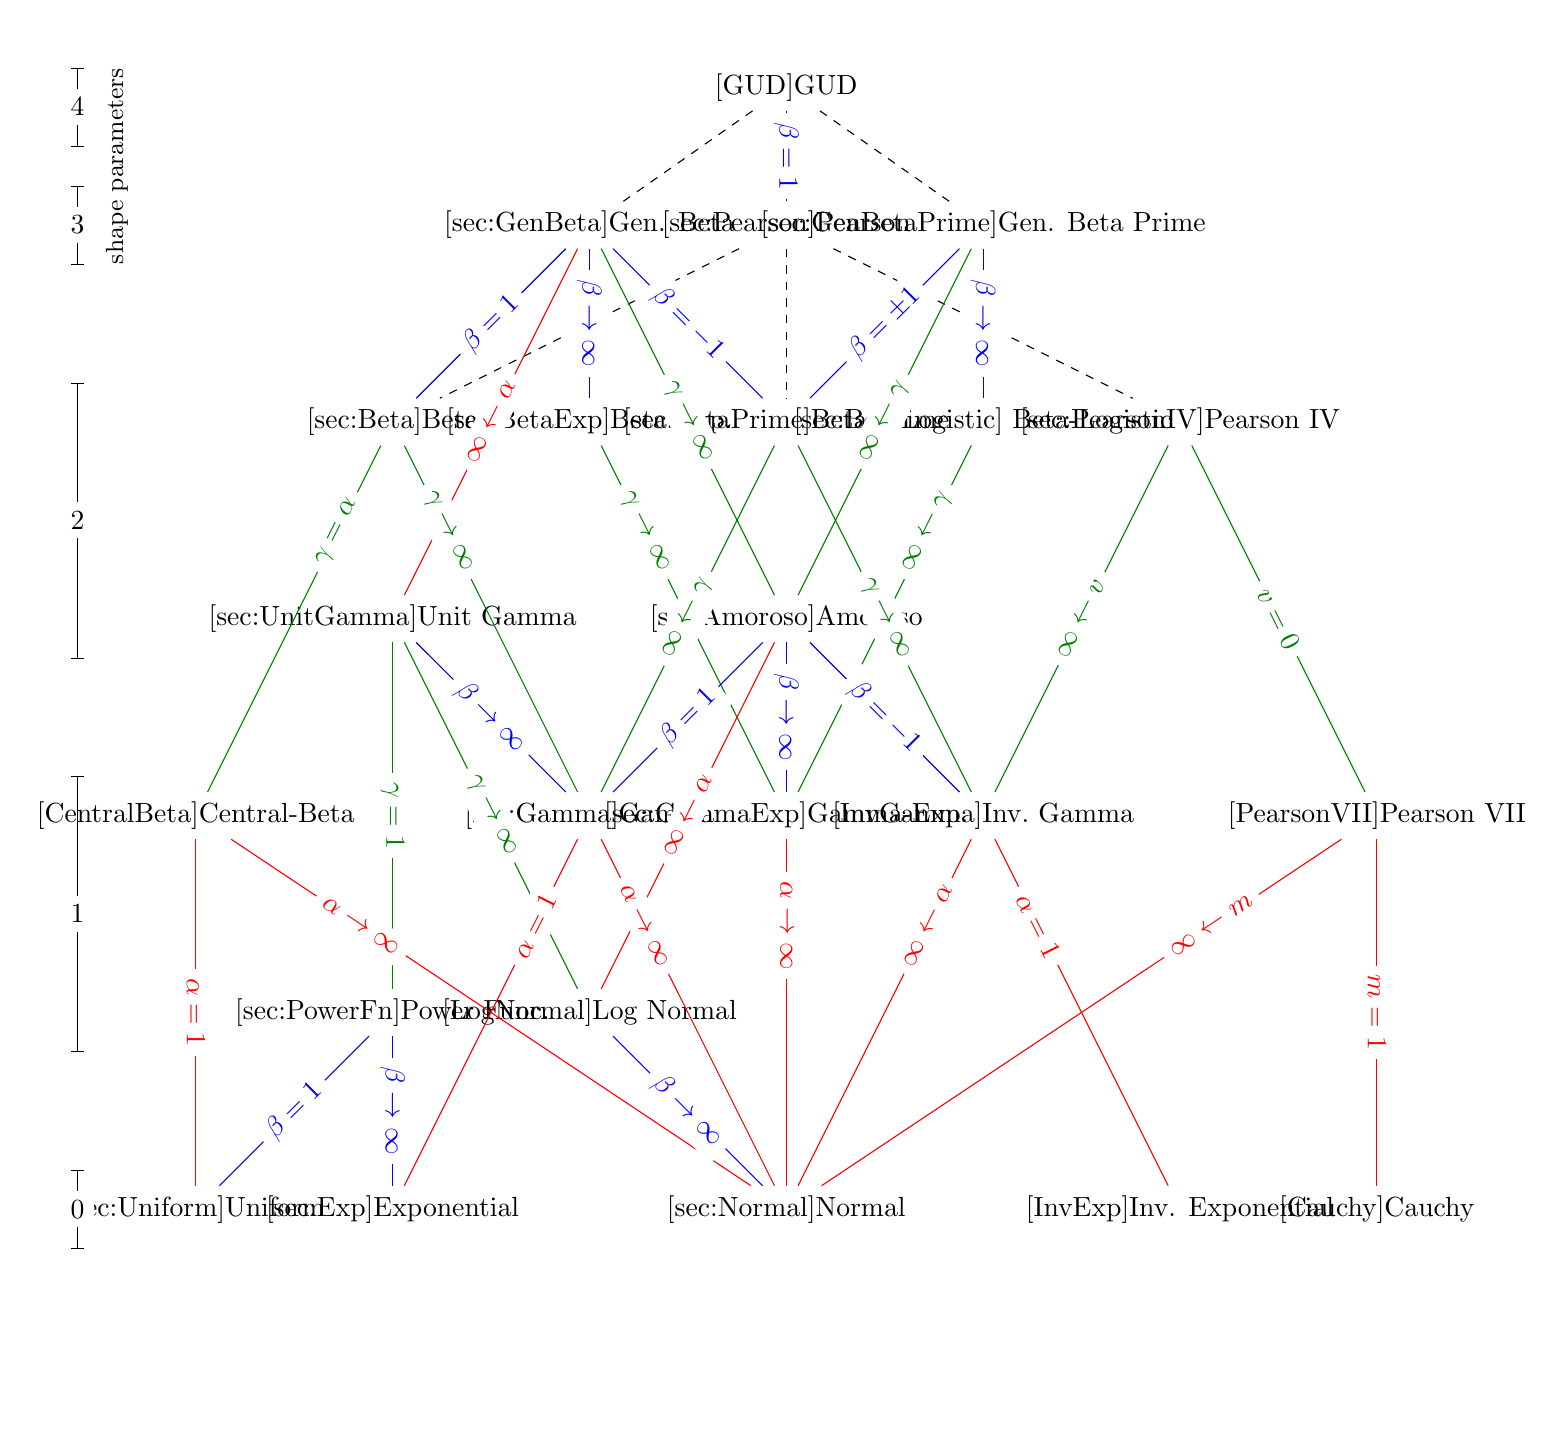
\begin{tikzpicture}
%\draw[help lines, very thin, step=1] (-2,0) grid (17,17);
%
\draw (7.5,16.75) node (gud) {\hyperref[GUD]{GUD}};
%
\draw (5,15) node (genbeta) {\hyperref[sec:GenBeta]{Gen. Beta}};
\draw (7.5,15) node (pearson) {\hyperref[sec:Pearson]{Pearson}};
\draw (10,15) node (genbetaprime) {\hyperref[sec:GenBetaPrime]{Gen. Beta Prime}};
%
\draw (2.5,12.5) node (beta) {\hyperref[sec:Beta]{Beta}};
\draw (5,12.5) node (betaexp) {\hyperref[sec:BetaExp]{Beta Exp.}};
\draw (7.5,12.5) node (betaprime) {\hyperref[sec:BetaPrime]{Beta Prime}};
\draw (10,12.5) node (betalogistic) {\hyperref[sec:BetaLogistic]{~Beta-Logistic}};
\draw (12.5,12.5) node (pearsoniv) {\hyperref[sec:PearsonIV]{Pearson IV}};
%
\draw (2.5,10) node (unitgamma) {\hyperref[sec:UnitGamma]{Unit Gamma}};
\draw (7.5,10) node (amoroso) {\hyperref[sec:Amoroso]{Amoroso}};
%\draw (12.5,10) node (burr) {\hyperref[Burr]{Burr}};
%
\draw (0,7.5) node  (pearsonii) {\hyperref[CentralBeta]{Central-Beta}};
\draw (2.5,5) node (power)  {\hyperref[sec:PowerFn]{Power Func.}};
\draw (5,7.5) node  (gamma) {\hyperref[sec:Gamma]{Gamma}};
\draw (7.5,7.5) node (gammaexp)  {\hyperref[sec:GammaExp]{Gamma-Exp.}};
\draw (10,7.5) node (invgamma) {\hyperref[InvGamma]{Inv.~Gamma}}; 
%\draw (12.5,7.5) node  (loglogistic) {\hyperref[LogLogistic]{Log-Logistic}};
\draw (15,7.5) node (pearsonvii) {\hyperref[PearsonVII]{Pearson VII }};
%
%\draw (5,5) node (weibull) {\hyperref[Weibull]{Weibull}};
%\draw (10,5) node (frechet) {\hyperref[Frechet]{Frechet}};
%\draw (12.5,7.5) node (lognormal) {\hyperref[LogNormal]{Log Normal}};
\draw (5,5) node (lognormal) {\hyperref[LogNormal]{Log Normal}};
%
\draw (0,2.5) node (uniform) {\hyperref[sec:Uniform]{Uniform}};
\draw (2.5,2.5) node (exp) {\hyperref[sec:Exp]{Exponential}};
%\draw (5,2.5) node (laplace) {\hyperref[sec:Laplace]{Laplace}};
\draw (7.5,2.5) node (normal) {\hyperref[sec:Normal]{Normal}};
%\draw (10,2.5) node (UniPrime) {\hyperref[Logistic]{Uniform Prime}};
%\draw (10,2.5) node (logistic) {\hyperref[Logistic]{Logistic}};
\draw (12.5,2.5) node (invexp) {\hyperref[InvExp]{Inv. Exponential}};
\draw (15,2.5) node (cauchy) {\hyperref[Cauchy]{Cauchy}};
%
%\draw (7.5,0) node (gumbel) {\hyperref[Gumbel]{Gumbel}};
%
\draw [dashed]  (gud) -- (genbeta);
\draw [blue]  (gud) -- (pearson) node [midway,  fill=white, sloped] (TextNode) {$\beta=1$} ;
\draw [dashed]  (gud) -- (genbetaprime);
%
\def\betaone{node}%
%
\draw [dashed]  (pearson) -- (beta);
\draw [dashed]  (pearson) -- (betaprime);
\draw [dashed]  (pearson) -- (pearsoniv);
%
\draw [blue]  (genbeta) --  (beta) node [midway,  fill=white, sloped] (TextNode) {$\beta=1$} ; 
\draw [blue]  (genbeta) --  (betaexp) node [midway,  fill=white, sloped] (TextNode) {$\beta\rightarrow\infty$} ;
\draw [blue]  (genbeta) --  (betaprime) node [midway,  fill=white, sloped] (TextNode) {$\beta=-1$} ;
\draw [red]  (genbeta) -- (unitgamma) node [fill=white, midway, sloped] (TextNode) {$\infty\leftarrow\alpha$} ;
\draw [darkgreen]  (genbeta) -- (amoroso)		node [midway, fill=white, sloped] (TextNode) {$\gamma\rightarrow\infty$} ;
%
\draw [blue]  (genbetaprime) -- (betalogistic) node [midway,  fill=white, sloped] (TextNode) {$\beta\rightarrow\infty$} ;
\draw [blue]  (genbetaprime) -- (betaprime) node [midway, fill=white, sloped] (TextNode) {$\beta=\pm1$} ;
\draw [darkgreen]  (genbetaprime) -- (amoroso) 	node [midway, fill=white, sloped] (TextNode) {$\infty\leftarrow\gamma$} ;
%\draw [dashed]  (genbetaprime) -- (burr);
%
\draw [darkgreen]  (beta) -- (pearsonii) node [near start,  fill=white, sloped] (TextNode) {$\gamma=\alpha$} ;
\draw [darkgreen]  (beta) -- (gamma) 	node [near start,  fill=white, sloped] (TextNode) {$\gamma\rightarrow\infty$} ;
%
\draw [darkgreen]  (betaexp) -- (gammaexp) node [near start,  fill=white, sloped] (TextNode) {$\gamma\rightarrow\infty$} ;
%
\draw [darkgreen]  (betaprime) -- (gamma)	node [midway, fill=white, sloped] (TextNode) {$\infty\leftarrow\gamma$} ;
%
\draw [darkgreen]  (betalogistic) -- (gammaexp) node [near start,  fill=white, sloped] (TextNode) {$\infty\leftarrow\gamma$} ;
\draw [darkgreen]  (betaprime) -- (invgamma)	node [midway, fill=white, sloped] (TextNode) {$\gamma\rightarrow\infty$} ;

%
\draw [darkgreen]  (pearsoniv) -- (invgamma) node [midway, fill=white, sloped] (TextNode) {$\infty\leftarrow v$} ;
\draw [darkgreen]  (pearsoniv) -- (pearsonvii)  node [midway, fill=white, sloped] (TextNode) {$v=0$} ;
\draw [darkgreen] (unitgamma) -- (power) node [midway,  fill=white, sloped] (TextNode) {$\gamma=1$} ;
\draw [blue]  (unitgamma) -- (gamma) node [midway,  fill=white, sloped] (TextNode) {$\beta\rightarrow\infty$} ;
%
\draw [blue]  (amoroso) -- (gamma) node [midway, fill=white, sloped] (TextNode) {$\beta=1$} ; 
%\draw [dashed]  (amoroso) -- (weibull);
\draw [blue]  (amoroso) -- (gammaexp) node [midway,  fill=white, sloped] (TextNode) {$\beta\rightarrow\infty$} ; 
\draw [blue]  (amoroso) -- (invgamma)	node [midway,  fill=white, sloped] (TextNode) {$\beta=-1$} ;
%\draw [dashed]  (amoroso) -- (frechet);
%
%\draw [dashed]  (burr) -- (frechet);
%\draw [dashed]  (burr) -- (loglogistic);
%
\draw [red]  (pearsonii) -- (uniform)	 node [midway, fill=white, sloped] (TextNode) {$\alpha=1$} ;
\draw [red]  (pearsonii) -- (normal) node [fill=white,  near start, sloped] (TextNode) {$\alpha\rightarrow\infty$} ;
\draw [blue]  (power) -- (uniform) 	 node [midway,  fill=white, sloped] (TextNode) {$\beta=1$} ;
\draw [blue]  (power) -- (exp) 			node [midway,  fill=white, sloped] (TextNode) {$\beta\rightarrow\infty$} ;
\draw [darkgreen] (unitgamma) -- (lognormal) node [midway,  fill=white, sloped] (TextNode) {$\gamma\rightarrow\infty$} ;	
\draw [red] (amoroso) -- (lognormal) node [midway,  fill=white, sloped] (TextNode) {$\infty\leftarrow\alpha$} ;

\draw [red]  (gamma) -- (exp)  node [near start, fill=white, sloped] (TextNode) {$\alpha=1$} ;
\draw [red]  (gamma) -- (normal) node [near start, fill=white, sloped] (TextNode) {$\alpha\rightarrow\infty$} ;
\draw [red]  (invgamma) -- (normal) node [near start, fill=white, sloped] (TextNode) {$\infty\leftarrow\alpha$} ;
\draw [red]  (invgamma) -- (invexp)  node [near start, fill=white, sloped] (TextNode) {$\alpha=1$} ;
%\draw [dashed]  (loglogistic) -- (logistic);
\draw [red]  (pearsonvii) -- (normal) node [near start, fill=white, sloped] (TextNode) {$\infty\leftarrow m$} ;
\draw [red]  (pearsonvii) -- (cauchy)  node [midway,  fill=white, sloped] (TextNode) {$m=1$} ;
%
%\draw [dashed]  (weibull) -- (exp);
%\draw [dashed]  (weibull) -- (gumbel);
%\draw [dashed]  (symbetalogistic) -- (laplace);
%\draw [dashed]  (symbetalogistic) -- (normal);
%\draw [dashed]  (symbetalogistic) -- (logistic);
%\draw [dashed]  (frechet) -- (gumbel);
%\draw [dashed]  (frechet) -- (invexp);
\draw [blue] (lognormal) -- (normal) node [midway, fill=white, sloped] (TextNode) {$\beta\rightarrow\infty$};
%
%\draw [dashed] (amoroso) -- +(5, -1.5)-- (lognormal);
%\draw [dashed] (gammaexp) -- +(0,-1) ;
%\draw [dashed] (gumbel) -- +(0,0.75) ;
%\draw [dashed] (gammaexp)  -- (gumbel) ;
\draw [red] (gammaexp)  -- (normal) node [near start, fill=white, sloped] (TextNode) {$\alpha\rightarrow\infty$} ;
%
%\draw (7.5,7.5) node[fill=white, fill opacity=0.75] {\hyperref[sec:GammaExp]{Gamma-Exp.}};
%
\draw[|-|, very thin] (-1.5,2) -- node[fill=white, midway] {0} (-1.5,3);
\draw[|-|, very thin]  (-1.5,4.5) -- node[fill=white, midway] {1} (-1.5,8);
\draw[|-|, very thin]  (-1.5,9.5) -- node[fill=white, midway] {2} (-1.5,13);
\draw[|-|, very thin]  (-1.5,14.5) -- node[fill=white, midway] {3} (-1.5,15.5);
\draw[|-|, very thin]  (-1.5,16) -- node[fill=white, midway] {4} (-1.5,17);
%
\draw (-1, 15.75) node[rotate=90]  {\small shape parameters};
%
\draw[white] (-2, 0) rectangle (17,17.5); % Bounding box
\end{tikzpicture}
}
\end{center}
\end{figure*}



 % =======================================================================
